% !TeX spellcheck = en_US	


\documentclass[10pt,journal,compsoc]{IEEEtran}
\usepackage{graphicx}
\usepackage[ruled, linesnumbered]{algorithm2e}
\usepackage{url}
\usepackage{epstopdf}
\usepackage{indentfirst}
\usepackage[tight,footnotesize]{subfigure}
\usepackage{amsmath}
\usepackage{amssymb}
\usepackage{multirow}
\usepackage{color}
\usepackage{enumerate}

\newtheorem{Formula}{Formula}
\newtheorem{Lemma}{Lemma}
\newtheorem{Corollary}{Corollary}
\newtheorem{Property}{Property}
\newtheorem{Rule}{Rule}

% *** CITATION PACKAGES ***
\ifCLASSOPTIONcompsoc
\usepackage[nocompress]{cite}
\else
\usepackage{cite}
\fi


\begin{document}


\title{Checking Big Suffix and LCP Arrays by Probabilistic Methods}

\author{
	Yi~Wu,
	Ge~Nong,
	Wai~Hong~Chan,
	Ling~Bo~Han% <-this % stops a space
	\IEEEcompsocitemizethanks{
		\IEEEcompsocthanksitem Y. Wu, G. Nong (corresponding author) and L.~B.~Han are with the Department of Computer Science, Sun Yat-sen University, Guangzhou 510275, China. E-mails: wu.yi.christian@gmail.com, issng@mail.sysu.edu.cn, hanlb@mail2.sysu.edu.cn.
		
		\IEEEcompsocthanksitem Wai Hong Chan (corresponding author) is with the Department of Mathematics and Information Technology, The Education University of Hong Kong, Hong Kong. E-mail: waihchan@ied.edu.hk.
}}% <-this % stops a space
	
\IEEEtitleabstractindextext{%
\begin{abstract}

For full-text indexing of massive data, the suffix and LCP (longest common prefix) arrays have been recognized as the fundamental data structures, and there are at least two needs in practice for checking their correctness, i.e. program debugging and verifying the arrays constructed by probabilistic algorithms. In this paper, we propose two methods to check the suffix and LCP arrays in external memory by using a Karp-Rabin fingerprinting technique, where the checking result is wrong only with a negligible error probability. The first method checks the lexicographical order and the LCP-value of two suffixes by computing and comparing the fingerprints of their LCPs. This method is of high versatility that it can verify any (sparse) suffix/LCP arrays of finite or infinite order. The second method is more space efficient, it first employs the same technique to verify a subset of the given suffix and LCP arrays, from which then a copy of the final suffix and LCP arrays is produced following the induced sorting principle and compared with the given arrays for verification.


\end{abstract}

% Note that keywords are not normally used for peerreview papers.
\begin{IEEEkeywords}
	Suffix and LCP arrays verification, Karp-Rabin fingerprinting technique, external memory.
\end{IEEEkeywords}}


% make the title area
\maketitle

\IEEEdisplaynontitleabstractindextext

\IEEEpeerreviewmaketitle

\section{Introduction}\label{sec:introduction}

\subsection{Background} \label{sec:introduction:background}


Suffix and longest common prefix (LCP) arrays play an important role in various string processing tasks, such as data compression, pattern matching and genome assembly. In many applications, these two data structures make up the core part of a powerful full-text index, called enhanced suffix array~\cite{Abouelhodaa2004}, which is more space efficient than a suffix tree and applicable to emulating any searching functionalities provided by the latter in the same time complexity. The first algorithm for building suffix array~(SA) in internal memory was presented in~\cite{Manber1993}. From then on, much more effort has been put on designing efficient constructors for suffix array on different memory models~\cite{Karkkainen2003, Ko2003, Kim2003, Nong11, Dementiev2008, Ferragina2012, Manzini2004, Bingmann12, Karkkainen2014, Nong14, Nong15}. In respect of the research on LCP array construction algorithms, the existing works can be classified into two categories with regard to their input requirements, where the algorithms from the first category compute both suffix and LCP arrays at the same time with the original text only~\cite{Fischer11, Bingmann12, Flick2015} and those from the second category carry out the computation by taking SA and/or Burrows-Wheeler transform (BWT) as additional input~\cite{Kasai2001,Karkkainen2009, Fischer11, Puglisi2008, Deo2013}. Among all, the algorithms designed by the induced sorting~(IS) principle take linear time and space to run and outperform previous arts on both internal and external memory models~\cite{Nong11, Karkkainen2014}. Recently, there appear some novel works that are competitive with the IS-based ones and can even achieve better performance when adequate computation resources are at hand. These algorithms are specific for parallel computation environments and capable of achieving high performance by fully using the available multi-core CPUs and/or GPUs~\cite{Osipov2012, Deo2013, Wang2015, Karkkainen2015, Karkkainen2016}. 

While the research on efficient construction of suffix and LCP arrays is evolving, the algorithms proposed recently are becoming more complicated than before. This reveals a need for program debugging because a program gives no guarantee that it has correctly implemented the underlying algorithm. As a common practice, a suffix or LCP checker is provided to check the correctness of a constructed array. For example, such a checker can be found in some software packages for SA-IS~\cite{Nong11}, eSAIS~\cite{Bingmann12}, DC3~\cite{Dementiev08} and so forth. In addition to help avoid implementation bugs, a checker is also demanded for an array constructed by a probabilistic algorithm~(e.g.~\cite{Bille2013}). In this case, the array is correctly constructed with a probability and hence must be verified by a checker to ensure its correctness. As far as we know, the work in~\cite{Burkhardt2003} describes the only SA checking method that can be found in the existing literature, and no efficient checking method for LCP array has been reported yet. Particularly, there is currently no reported solution that can check both the suffix and the LCP arrays in external memory. This motivates our work here to design high-performance checkers for massive data.  
	
\subsection{Contribution}\label{sec:introduction:contribution}

Our contribution mainly includes two methods to probabilistically verify the given suffix and LCP arrays. Method A checks the lexical order and the LCP-value of two neighboring suffixes in SA by literally comparing the characters of their LCPs in pairs. For reducing the time complexity of a comparison between two sequences of characters, we use a Karp-Rabin fingerprinting technique to convert each sequence into a single integer, called fingerprint, and compare the fingerprints instead to check equality of these sequences. The algorithm for Method A involves multiple scans and sorts on sets of $\mathcal{O}(n)$ fixed-size items. When implemented in external memory, it suffers from a space bottleneck owing to the large disk volume taken by each sort. 
To overcome the drawback, Method B first employs the fingerprinting technique to check a subset selected from the given suffix and LCP arrays, then it reuses the inducing process of an IS-based construction algorithm to produce the final suffix and LCP arrays from the verified subset and literally compares them with the input arrays to ensure the correctness of the latter. Our experiments indicate that the peak disk use of the programs for Algorithm~\ref{alg:2} designed by Method B is only about half as that of the program for Algorithm~\ref{alg:1} designed by Method A.

The remainder of this paper is organized as follows. We first describe the two methods and their algorithmic designs in Sections~\ref{sec:method1} and~\ref{sec:method2}, and then the evaluation of our programs for the algorithms designed by these methods in Section~\ref{sec:experiment}. Finally, we present the concluding remarks in Section~\ref{sec:conclusion}. 



\section{Method A} \label{sec:method1}


\subsection{Preliminaries} \label{sec:method1:notations}

Given a string $x[0, n)$ drawn from an alphabet $\Sigma$, the suffix array of $x$, denoted by $sa$, is a permutation of $\{0, 1, ..., n - 1\}$ such that ${\sf suf}(sa[i]) < {\sf suf}(sa[j])$ for $i, j \in [0, n)$ and $i < j$, where ${\sf suf}(sa[i])$ and ${\sf suf}(sa[j])$ are two suffixes starting with $x[sa[i]]$ and $x[sa[j]]$, respectively. Particularly, we say ${\sf suf}(sa[j])$ is a lexical neighbor of ${\sf suf}(sa[i])$ if $|i - j| = 1$. The LCP array of $x$, denoted by $lcp$, consists of $n$ integers, where $lcp[0]=0$ and $lcp[i]$ records the LCP-value of ${\sf suf}(sa[i])$ and ${\sf suf}(sa[i - 1])$ for $i \in [1, n)$. 

\subsection{Idea} \label{sec:method1:idea}

According to the above definitions, we show in Lemma~\ref{lemma:1} the sufficient and necessary conditions for checking suffix and LCP arrays. Notice that the lexical order and the LCP-value of any two suffixes in $x$ can be computed by literally comparing their characters rightward. To do this, we assume $x[n]$ to be an empty character lexicographically smaller than any characters of $\Sigma$. Because all the suffixes differ in length and end with the empty character, there must exist $k \in [0, n)$ such that $x[i, i + k) = x[j, j + k)$ and $x[i + k] \ne x[j + k]$ for $i, j \in [0, n)$ and $i \ne j$. This approach can be also applied to verifying the last two conditions in Lemma~\ref{lemma:1}, but it takes at worst $\mathcal{O}(n)$ character-wise comparisons for each pair of neighboring suffixes in $sa$ to compare the underlying substrings indicated by their LCP-value.

\begin{Lemma} \label{lemma:1}
	Both $sa[0, n)$ and $lcp[0, n)$ are correct if and only if the following conditions are satisfied, for all $i \in [1, n)$:
	\begin{enumerate}[(1)]
		\item
		$sa$ is a permutation of $\{0, 1, \dots, n - 1\}$.
		\item
		$x[sa[i], sa[i] + lcp[i] - 1] = x[sa[i - 1], sa[i - 1] + lcp[i] - 1]$.
		\item
		$x[sa[i] + lcp[i]] > x[sa[i - 1] + lcp[i]]$. 	
	\end{enumerate}
\end{Lemma}

\begin{IEEEproof}
	Both the sufficiency and necessity are immediately seen from the definition of suffix and LCP arrays. Specifically, condition (1) demonstrates that all the suffixes in $x$ are sorted in $sa$, while conditions (2)-(3) indicate that the lexical order and the LCP-value of any two neighboring suffixes in $sa$ are both correct.
\end{IEEEproof}

An alternative is to exploit a perfect hash function~(PHF) to convert each substring into a single integer such that any two substrings have a common hash value if and only if they are literally equal to each other. This implies that we can compare the hash values of substrings instead to check their equality. The key point here is how to quickly calculate the hash values of $x[sa[i], sa[i] + lcp[i] - 1]$ and $x[sa[i - 1], sa[i - 1] + lcp[i] - 1]$ for all $i \in [1, n)$. Taking into account the high difficulty of finding a PHF to meet this requirement, we prefer using a Karp-Rabin fingerprinting function~\cite{Karp1987} to transform a substring into its integer form, called fingerprint. To be specific, suppose $L$ is a prime and $\delta$ is a number randomly chosen from $[1, L)$, the fingerprint ${\sf fp}(i, j)$ for a substring $x[i, j]$ can be calculated according to the formulas below as following: scan $x$ rightward to iteratively compute ${\sf fp}(0, k)$ for all $k \in [0, n)$ using Formulas~\ref{formula:1}-\ref{formula:2}, record ${\sf fp}(0, i - 1)$ and ${\sf fp}(0, j)$ during the calculation and subtract the former from the latter to obtain ${\sf fp}(i, j)$ using Formula~\ref{formula:3}.

\begin{Formula} \label{formula:1}
	${\sf fp}(0, -1) = 0$.
	
\end{Formula}

\begin{Formula} \label{formula:2}	
	${\sf fp}(0, i) = {\sf fp}(0, i - 1) \cdot {\delta} + x[i]\mod L$ for $i \ge 0$.
	
\end{Formula}

\begin{Formula} \label{formula:3}
	${\sf fp}(i, j) = {\sf fp}(0, j) - {\sf fp}(0 ,i - 1) \cdot {\delta}^{j - i + 1}\mod L$.
	
\end{Formula}

We point out that two equal substrings always share a common fingerprint, but the inverse is not true. Fortunately, it has been proved in~\cite{Karp1987} that the probability of a false match can be reduced to a negligible level by setting $L$ to a large value\footnote{This property is utilized in~\cite{Bille2013} to design a probabilistic algorithm for computing a sparse suffix array. }. This leads us to the conclusion in Corollary~\ref{corollary:1}.

\begin{Corollary} \label{corollary:1}
	Both $sa[0, n)$ and $lcp[0, n)$ are correct with a high probability given the following conditions, for all $i \in [1, n)$:
	
	\begin{enumerate}[(1)]
		\item
		$sa$ is a permutation of $\{0, 1, \dots, n - 1\}$.
		
		\item
		${\sf fp}(sa[i], sa[i] + lcp[i] - 1) = {\sf fp}(sa[i - 1], sa[i - 1] + lcp[i] - 1)$.
		
		\item
		$x[sa[i] + lcp[i]] > x[sa[i - 1] + lcp[i]]$.
	\end{enumerate}
\end{Corollary}

We close this part with an example in Fig.~\ref{fig:example} for a better understanding. Given that $L = 197$ and $\delta = 101$, lines 4-8 compute ${\sf fp}(0, p)$ iteratively according to Formulas~\ref{formula:1}-\ref{formula:2}. Then, lines 10-16 use these values to compute the fingerprints for all the target substrings. Consider the leftmost pair of neighboring suffixes in $sa$, that is ${\sf suf}(sa[0])$ and ${\sf suf}(sa[1])$, the substrings indicated by their LCP-value are $x[sa[0], sa[0] + lcp[1] - 1]$ and $x[sa[1], sa[1] + lcp[1] - 1]$, respectively. According to Formula~\ref{formula:3}, ${\sf fp}(sa[0], sa[0] + lcp[1] - 1)$ is equal to the difference between ${\sf fp}(0, sa[0] - 1)$ and ${\sf fp}(0, sa[0] + lcp[1] - 1)$, both of which have been calculated beforehand. Following the same way, ${\sf fp}(sa[1], sa[1] + lcp[1] - 1)$ is computed by deducting ${\sf fp}(0, sa[1] - 1)$ from ${\sf fp}(0, sa[1] + lcp[1] - 1)$. Hence, we obtain the fingerprints for these two substrings in lines 10-12 and see that they are equal to each other. 

\begin{figure}
	\centering
	
	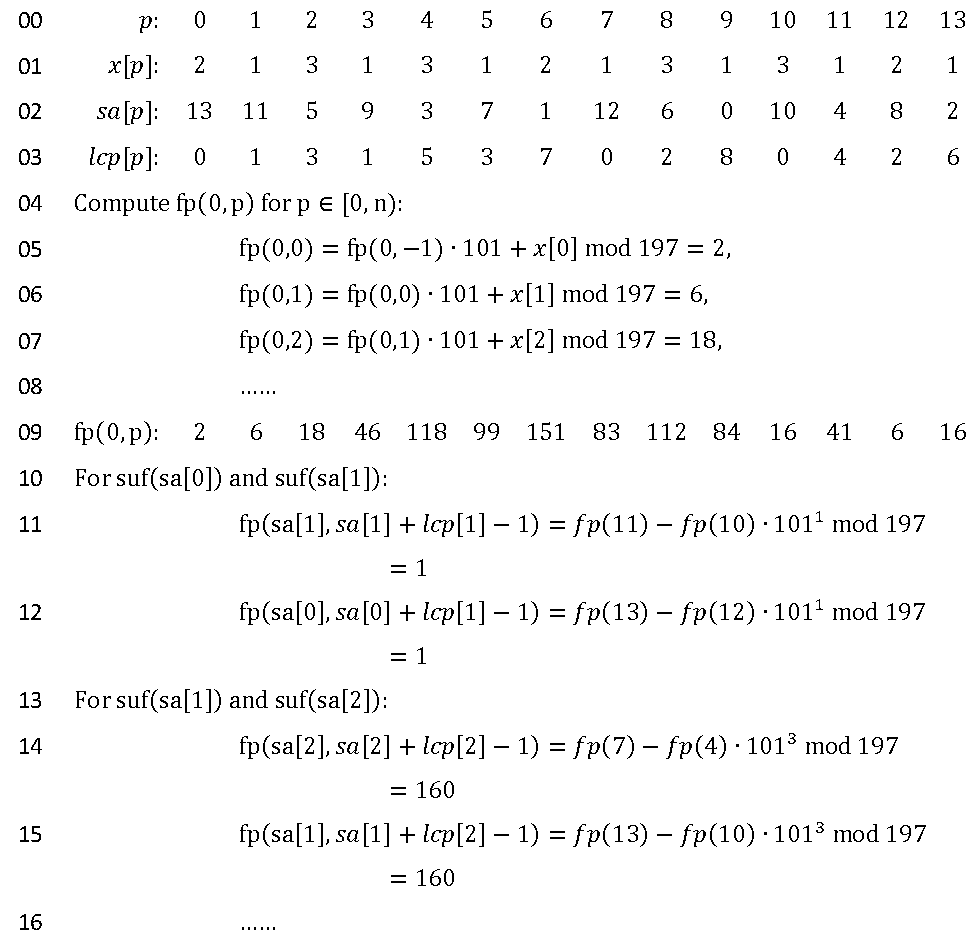
\includegraphics[width = 0.9\columnwidth]{example}
	\caption{An Example for Computing and Comparing Fingerprints for Substrings Specifed by the LCP-Values of Neighboring Suffixes in SA. \label{fig:example}}	
\end{figure}

\subsection{Algorithm} \label{sec:method1:algorithm}

We describe an algorithm for checking the conditions in Corollary~\ref{corollary:1} on random access models, of which the core part is to check the lexical order and the LCP-value for each pair of neighboring suffixes in $sa$ on-the-fly during the scan of $sa$ and $lcp$. This is done by using Formulas~\ref{formula:1}-\ref{formula:3} following our discussion in the previous subsection. Two zero-initialized array, namely $fp$ and $mk$, are introduced to facilitate the checking process, where $fp$ is for storing the fingerprints of all the prefixes in $x$ and $mk$ is for checking whether or not each number of $\{0, 1, ..., n - 1\}$ is present in $sa$.

\begin{enumerate}
	\item [S1]
	Scan $x$ rightward with $i$ increasing from $0$ to $n - 1$. For each scanned $x[i]$, compute ${\sf fp}(0, i)$ and assign the value to $fp[i]$.
	
	\item [S2]
	Scan $sa$ and $lcp$ rightward with $i$ increasing from $1$ to $n - 1$. For each scanned $sa[i]$ and $lcp[i]$, let $u = sa[i], v = lcp[i], w = sa[i - 1]$ and perform substeps (a)-(c) in sequence:
	
	\begin{enumerate}[(a)]
		\item
		Retrieve $fp[u - 1]$ and $fp[u + v - 1]$ from $fp$ to compute ${\sf fp}(u, u + v - 1)$. Set $mk[u]$ to $1$.
		
		\item
		Retrieve $fp[w - 1]$ and $fp[w + v - 1]$ from $fp$ to compute ${\sf fp}(w, w + v - 1)$.
		
		\item
		Check if ${\sf fp}(u, u + v - 1) = {\sf fp}(w, w + v - 1)$ and $x[u + v] > x[w + v]$.
		
		\item
		Set $mk[sa[0]] = 1$.
	\end{enumerate}

	\item [S3] Check if $mk[i] = 1$ for all $i \in [0, n)$.
	
\end{enumerate}

It is clear that the above algorithm consumes $\mathcal{O}(n)$ time and space when implemented in internal memory. However, if the two auxiliary arrays cannot be wholly accommodated into RAM during the execution of S2, it suffers from a performance degradation caused by frequent random accesses to disks. Assume that $x$, $sa$ and $lcp$ are stored in external memory, we design Algorithm~\ref{alg:1} for conducting these I/O operations in a disk-friendly way. The main idea is to first sort data in the order that they are to be visited and then access them by sequential reads. For the purpose, Algorithm~\ref{alg:1} first scans $sa$ and $lcp$ to produce $ST_1, ST_2, ST_3$ and sorts their tuples by 1st component in ascending order at the very beginning (lines~\ref{alg:1:a}-\ref{alg:1:b}). Afterward, it iteratively computes the fingerprints of all the prefixes according to Formulas~\ref{formula:1}-\ref{formula:2} and assigns them to the sorted tuples as following (lines~\ref{alg:1:c}-\ref{alg:1:d}): when figuring out ${\sf fp}(0, i - 1)$, extract each tuple $e$ with $e.1st = i$ from $ST_1/ST_2/ST_3$, update $e$  with ${\sf fp}(0, i - 1)$, and then forward $e$ to $ST_1'/ST_2'/ST_3'$. Because the 1st components of the tuples in $ST_1$ constitute a copy of $sa$, the algorithm checks condition (1) when scanning these tuples in their sorted order. Finally, it sorts the updated tuples back to their original order~(line~\ref{alg:1:e}) and visits them  sequentially to check conditions (2)-(3) following the same way of S2~(lines~\ref{alg:1:f}-\ref{alg:1:g}).  



\SetKwProg{Fn}{Function}{}{}

\begin{algorithm*}

	\caption{The Algorithm Based on Corollary~\ref{corollary:1}.}
	
	\label{alg:1}
	
	%\SetAlgoNoLine
	\Fn{{\sf CheckByFP}($x$, $sa$, $lcp$, $n$)}{
	
		$ST_1$ := $[(sa[i], i, null) | i \in [0, n)]$ \label{alg:1:a}
		
		$ST_2$ := $[(sa[i] + lcp[i + 1], i, null, null) | i \in [0, n - 1)]$
			
		$ST_3$ := $[(sa[i] + lcp[i], i, null, null) | i \in [1, n)]$
		
		sort tuples in $ST_1$, $ST_2$ and $ST_3$ by 1st component \label{alg:1:b}
		
		$fp := 0$  \label{alg:1:c}
		
		\For{$i \in [0, n]$}{
			
			\If{$ST_1.{\sf notEmpty}()$ {\sf and} $ST_1.{\sf top}().1st = i$}{~\label{alg:1:h}
				$e := ST_1.{\sf top}()$, $ST_1.{\sf pop}()$, $e.3rd := fp$, $ST_1'.{\sf push}(e)$
			}
			\Else{
				\Return false \hspace{5cm} // condition (1) is violated
			}~\label{alg:1:i}
			\While{$ST_2.{\sf notEmpty}()$ {\sf and} $ST_2.{\sf top}().1st = i$}{
				
				$e := ST_2.{\sf top}()$, $ST_2.{\sf pop}()$, $e.3rd := fp$, $e.4th := x[i]$, $ST_2'.{\sf push}(e)$
			}	
		
			\While{$ST_3.{\sf notEmpty}()$ {\sf and} $ST_3.{\sf top}().1st = i$}{
				
				$e := ST_3.{\sf top}()$, $ST_3.{\sf pop}()$, $e.3rd := fp$, $e.4th := x[i]$, $ST_3'.{\sf push}(e)$
			}	
		
			$fp := fp \cdot \delta + x[i] \! \mod \! P$
		} \label{alg:1:d}
		
		sort tuples in $ST_1'$, $ST_2'$ and $ST_3'$ by 2nd component.  \label{alg:1:e}
		
		\For {$i \in [1, n)$}{  \label{alg:1:f}
			
			$fp_1 := ST_1'.{\sf top}().3rd$, $ST_1'.{\sf pop}()$, $fp_2 := ST_2'.{\sf top}().3rd$, $ch_1 := ST_2'.{\sf top}().4th$, $ST_2'.{\sf pop}()$
			
			$\hat{fp_1} = fp_2 - fp_1 \cdot \delta^{lcp[i]} \! \mod \! P$ \label{alg:1:j}
		
		 	$fp_1 := ST_1'.{\sf top}().3rd$, $fp_3 := ST_3'.{\sf top}().3rd$, $ch_2 := ST_3'.{\sf top}().4th$, $ST_3'.{\sf pop}()$
			
			$\hat{fp_2} = fp_3 - fp_1 \cdot \delta^{lcp[i]} \! \mod \! P$	\label{alg:1:k}
			
			\If{$\hat{fp_1} \ne \hat{fp_2}$ {\sf or} $ch_1 \le ch_2$}{
				
				\Return false \hspace{5cm} // condition (2) or (3) is violated
			}	
		} \label{alg:1:g}

		\Return true
	}
	\end{algorithm*}

The last point to be mentioned here is how to obtain the value of $\delta^{lcp[i]}$ quickly when computing $\hat{fp_1}$ and $\hat{fp_2}$ in lines~\ref{alg:1:j} and~\ref{alg:1:k}. One method is to keep a lookup table in internal memory to store $\delta^{lcp[i]}$ for all $i \in [0, n)$. This method can answer the question in constant time, but it is space-consuming and 
impractical to use if the table size exceeds the capacity of memory bank. We provide another method that returns the answer in $\mathcal{O}(\lceil \log2^n \rceil)$ time using $\mathcal{O}(\lceil \log2^n \rceil)$ internal memory space. Specifically, suppose $e$ is an integer from $[0, n)$, it can be broken down into the form of $\Sigma_{i = 0}^{\lceil \log2^n \rceil}{k_i \cdot 2^i}$ by performing at most $\lceil \log2^n \rceil$ divisions, where $k_0, k_1, ..., k_{\lceil \log2^n \rceil}$ are integers from $\{0, 1\}$ . Thereby, we have $\delta^e = \Pi_{i = 0}^{\lceil \log2^n \rceil}{\delta}^{k_i \cdot 2^i}$ by replacing $e$ with its decomposition, where the expression on the right side of the equation can be easily computed with $\{{\delta}^{1}, {\delta}^{2}, \dots, {\delta}^{2^{\lceil \log2^n \rceil}} \}$ already known.

\subsection{Analysis} \label{sec:method1:analysis}


Algorithm~\ref{alg:1} is I/O-intensive, it performs multiple scans and sorts on the arrays of $\mathcal{O}(n)$ fixed-size tuples residing on disks. Given an external memory model with RAM size $M$, disk size $D$ and block size $B$, all are in words, the time and I/O complexities for each scan are $\mathcal{O}(n)$ and $\mathcal{O}(n / B)$, respectively, while those for each sort are $\mathcal{O}(n\log_{M/ B}(n / B))$ and $\mathcal{O}((n / B)\log_{M / B}(n / B))$, respectively~\cite{Arge2013}. Clearly, this algorithm reaches its peak disk use when sorting tuples in lines~\ref{alg:1:b} and~\ref{alg:1:e}. The experimental study in Section~\ref{sec:experiment} indicates that our program for Algorithm~\ref{alg:1} is rather space consuming, its peak disk use reaches 40 bytes per input character.

\section{Method B} \label{sec:method2}

\subsection{Preliminaries} \label{sec:method2:preliminaries}

In this part, we describe an alternative checking method based on the induced sorting principle. Compared with Algorithm~\ref{alg:1}, our programs for Algorithm~\ref{alg:2} designed by this method take around half disk space on real-world datasets. Before the presentation, we introduce some symbols and notations used in the following paragraphs.

{\em Character and suffix classification.} All the characters in $x$ are classified into three types, namely L-, S- and S*-type. In detail, $x[i]$ is L-type if (1) $i = n - 1$ or (2) $x[i] > x[i + 1]$ or (3) $x[i] = x[i + 1]$ and $x[i + 1]$ is L-type; otherwise, $x[i]$ is S-type. Further, if $x[i]$ and $x[i + 1]$ are separately L-type and S-type, then $x[i + 1]$ is also an S*-type character. Moreover, a suffix is L-, S- or S*-type if its heading character is L-, S-, or S*-type, respectively.

{\em Suffix and LCP buckets.} Suppose $sa$ is correct, all the suffixes in $sa$ are naturally partitioned into multiple buckets and those of a common heading character are grouped into a single bucket that occupies a contiguous interval in $sa$. Each bucket can be further divided into two sub-buckets, where the left and the right parts only contain L- and S-type suffixes, respectively. For short, we use ${\sf sa\_bkt}(c)$ to denote the bucket storing suffixes starting with character $c$ and ${\sf sa\_bkt_L}(c)/{\sf sa\_bkt_S}(c)$ to denote its left/right sub-bucket. Accordingly, $lcp$ can be also split into multiple buckets, where ${\sf lcp\_bkt}(c)/{\sf lcp\_bkt_L}(c)/{\sf lcp\_bkt_S}(c)$ stores the LCP-values of suffixes in ${\sf sa\_bkt}(c)/{\sf sa\_bkt_L}(c)/{\sf sa\_bkt_S}(c)$.

{\em Suffix and LCP arrays for S*-type suffixes.} Given that the number of S*-type suffixes is $n_1$, $sa^*[0, n_1)$ stores all the S*-type suffixes arranged in lexical order, while $lcp^*[0] = 0$ and $lcp^*[i]$ records the LCP-value of ${\sf suf}(sa^*[i])$ and ${\sf suf}(sa^*[i - 1])$ for $i \in [1, n_1)$.

{\em Type Array.} The array $t$ records in $t[i]$ the type information of $x[i]$, where $t[i] = 1$ or $0$ if $x[i]$ is S-type or L-type, respectively.

\subsection{Idea} \label{sec:method2:idea}

The induced sorting principle has been extensively used to design efficient algorithms for constructing the suffix and LCP arrays on internal and external memory models. An IS-based construction algorithm mainly consists of a reduction phase for computing $sa^*$ and $lcp^*$, followed by an induction phase for inducing $sa$ and $lcp$ from $sa^*$ and $lcp^*$~\footnote{In the interest of completeness, we give an overview of the induction phase in Appendix~\ref{sec:appendix}.}. Given that $sa^*$ and $lcp^*$ are already known, we can produce the final suffix and LCP arrays by calling the inducing process of an existing IS-based construction algorithm. This enlightens us to design a checker based on Lemma~\ref{lemma:2}. 
	
\begin{Lemma} \label{lemma:2}
Both $sa[0, n)$ and $lcp[0, n)$ are correct if and only if the conditions below are satisfied:

\begin{enumerate}[(1)]
	\item
	$sa^*$ and $lcp^*$ are both correct.
	\item
	$sa = sa'$ and $lcp = lcp'$, where $sa'$ and $lcp'$ are induced from $sa^*$ and $lcp^*$ by calling the inducing process of an existing IS-based construction algorithm.
\end{enumerate}
\end{Lemma}

Similar to Method A, we can employ the fingerprinting technique to probabilistically check the correctness of $sa^*$ and $lcp^*$. Based on this idea, we describe in the next subsection an external-memory algorithm for checking the conditions in Corollary~\ref{corollary:2}.

\begin{Corollary} \label{corollary:2}
Both $sa[0, n)$ and $lcp[0, n)$ are correct with a high probability given the following conditions:
	
\begin{enumerate}[(1)]
	\item
	$x[sa^*[i]]$ is S*-type and $sa^*[i] \ne sa^*[j]$ for $i, j \in [0,n_1)$ and $i \ne j$.
	\item
	${\sf fp}(sa^*[i], sa^*[i] + lcp^*[i] - 1) = {\sf fp}(sa^*[i - 1], sa^*[i - 1] + lcp^*[i] - 1)$ for $i \in [1, n_1)$.
	\item
	$x[sa^*[i] + lcp^*[i]] > x[sa^*[i - 1] + lcp^*[i]]$ for $i \in [1, n_1)$.
	\item
	$sa[i] = sa'[i]$ and $lcp[i] = lcp'[i]$ for $i \in [0, n)$, where $sa'$ and $lcp'$ are induced from $sa^*$ and $lcp^*$ by calling the inducing process of an existing IS-based construction algorithm.
\end{enumerate}

\end{Corollary}


\subsection{Algorithm} \label{sec:method2:algorithm}

The first step of Algorithm~\ref{alg:2} is to compute and verify $sa^*$ and $lcp^*$. According to their definitions, $sa^*$ can be produced by sequentially retrieving the S*-type suffixes from $sa$ and the LCP-value of two successive S*-type suffixes in $sa$, say ${\sf suf}(sa[i])$ and ${\sf suf}(sa[j])$, is equal to the minimal of $\{lcp[i + 1], ..., lcp[j - 1], lcp[j]\}$. Hence, the proposed algorithm first sorts all the suffixes in $sa$ by their starting positions~(lines~\ref{alg:2:a}-\ref{alg:2:b}) and then scans $x$ only once to pick out the S*-type suffixes~(lines~\ref{alg:2:c}-\ref{alg:2:d}). After that, it puts these S*-type suffixes back in their lexical order and outputs them one by one to generate $sa^*$~(lines~\ref{alg:2:g}-\ref{alg:2:h}). Meanwhile, it calculates the LCP-value for each pair of the neighboring suffixes in $sa^*$ by tracing the minimal over the $lcp$ interval indicated by the two suffixes. Notice that, we check condition (1) in Corollary~\ref{corollary:2} during the time when visiting the suffixes in position order (lines~\ref{alg:2:e}-\ref{alg:2:f}) and conditions (2)-(3) by calling Algorithm~\ref{alg:1} with $sa^*$ and $lcp^*$ as input. Suppose $sa^*$ and $lcp^*$ are both correct, then Algorithm~\ref{alg:2} invokes the inducing process of an existing IS-based construction algorithm to induce $sa'$ and $lcp'$, which are a copy of the final suffix and LCP arrays, from the two verified arrays~(line~\ref{alg:2:k}) and literally compares them with $sa$ and $lcp$ to complete the whole checking process~(lines~\ref{alg:2:l}-\ref{alg:2:m}).

\begin{algorithm*}[!htbp]
	
	\caption{The Algorithm Based on Corollary~\ref{corollary:2}.}
	
	\label{alg:2}
	
	%\SetAlgoNoLine
	\Fn{{\sf CheckByIS}($x$, $sa$, $lcp$, $n$)}{	
	
	$ST_1$ := $[(sa[i], i, null) | i \in [0, n)]$ \label{alg:2:a}
		
	sort tuples in $ST_1$ by 1st component \label{alg:2:b}
	
	$pos := -1$ \label{alg:2:c}
	
	\For{$i \in (n, 0]$}{
	
		$e := ST_1.{\sf top}()$, $ST_1.{\sf pop}()$
		
		\If{$x[i]$ is S*-type}{ \label{alg:2:e}
			
			\If{$pos \ge e.1st$}{
			
				\Return false  \hspace{1cm} // condition (1) is violated
			}
		
			$ST_2.{\sf push}(e)$, $pos := e.1st$
		}\label{alg:2:f}
	} \label{alg:2:d}

	sort tuples in $ST_2$ by 2nd component \label{alg:2:g}
	
	$i := 0$, $j := 0$, $lcp_{min} := max\_val$
	
	\While{$ST_2.{\sf NotEmpty()}$}{
	
		$e := ST_2.{\sf top}()$, $ST_2.{\sf pop}()$
	
		\While {true} {
			
			$lcp_{min} := {\sf min}(lcp_{min}, lcp[i])$
			
			\If {$e.2nd = i$} {
			
				$sa^*[j] := e.1st$, $lcp^*[j] := lcp_{min}$, $j := j + 1$, $i:= i + 1$
				
				\textbf{break}
			}
			
			$i:= i + 1$
		}
	
		$lcp_{min} := max\_val$
	} \label{alg:2:h}
	
	\If{${\sf CheckByFP}(x, sa^*, lcp^*, n_1) = false$}{  \label{alg:2:i}
	
		\Return false \hspace{1cm} // conditions (2) or (3) is violated
	}\label{alg:2:j}

	$(sa', lcp') := {\sf InducingProcess}(x, sa^*, lcp^*)$ \label{alg:2:k}
	
	\For{$i \in [0, n)$}{\label{alg:2:l}
	
		\If{$sa[i] \ne sa'[i] \parallel lcp[i] \ne lcp'[i]$}{
		
			\Return false \hspace{1cm}	// condition (4) is violated
		}	
	}\label{alg:2:m}

	\Return true
}
\end{algorithm*}

Assume that the alphabet $\Sigma$ is of a constant size, we can check $sa$ and $lcp$ without producing a copy of the final suffix and LCP arrays in Algorithm~\ref{alg:2}. The idea is to compare the induced suffix/LCP items with their corresponding items in $sa/lcp$ during the inducing process. Specifically, when a suffix/LCP item $v_1$ is induced into a bucket, we check if it is equal to the corresponding item $v_2$ in $sa/lcp$. If $v_1 = v_2$, then $v_2$ is correct and we further use this value to induce the remaining suffix/LCP items. The key point here is to retrieve items of $sa/lcp$ from external storage as fast as possible. This can be done by conducting sequential I/O operations if we provide a read pointer together with a buffer for each suffix/LCP sub-bucket. We describe below more details of the adapted inducing process, where $lp_1/lp_2$ and $sp_1/sp_2$ are file pointer arrays for reading items from the sub-buckets of $sa$ and $lcp$.

\begin{enumerate}
	\item [S1]
	\begin{enumerate}[(a)]
		\item 
		Let $lp_1[c]$ and $lp_2[c]$ point to the leftmost items of ${\sf sa\_bkt_L}(c)$ and ${\sf lcp\_bkt_L}(c)$, for $c \in [0, \Sigma)$.
		\item 
		Scan $sa$ and $lcp$ rightward to induce L-type suffixes and their LCP-values. For each induced suffix $p$ (with a heading character $c_0$) and its LCP-value $q$: (1) check if $p = lp_1[c_0]$ and $q = lp_2[c_0]$; (2) move $lp_1[c_0]$ and $lp_2[c_0]$ to the next items on the right.
	\end{enumerate}
	\item [S2]
	\begin{enumerate}[(a)]
		\item 	
		Let $sp_1[c]$ and $sp_2[c]$ point to the rightmost items of ${\sf sa\_bkt_S}(c)$ and ${\sf lcp\_bkt_S}(c)$, for $c \in [0, \Sigma)$.
		\item 	
		Scan $sa$ and $lcp$ leftward to induce S-type suffixes and their LCP-values. For each induced suffix $p$ (with a heading character $c_0$) and its LCP-value $q$: (1) check if $p = sp_1[c_0]$ and $q = sp_2[c_0]$; (2) move $sp_1[c_0]$ and $sp_2[c_0]$ to the next items on the left.
	\end{enumerate}
\end{enumerate}

\subsection{Analysis} \label{sec:method2:analysis}

Algorithm~\ref{alg:2} mainly consists of two parts, where the first part for checking $sa^*$ and $lcp^*$ can be implemented within sorting complexity and the second part for checking $sa$ and $lcp$ can be implemented in linear time. As will be seen from Section~\ref{sec:experiment}, the peak disk use of our program for the optimized version of Algorithm~\ref{alg:2} is around $21n$ under the condition of $\|\Sigma\| = \mathcal{O}(1)$, and it even runs faster than the program for Algorithm~\ref{alg:1} in some cases.

\section{Experiments} \label{sec:experiment}

\subsection{Setup} \label{sec:experiment:setup}

For implementation simplicity, our programs for the algorithms proposed in the previous sections use the external-memory containers provided by the STXXL library~\cite{Dementiev2007} to manage read/write operations on disks. We make a performance evaluation by running them on the real-world corpora listed in Table~\ref{tbl:1}, where three measures normalized by the size of input string are investigated:

\begin{itemize}
	
	\item RT: running time, in microseconds.
	
	\item PDU: peak disk use of external memory, in bytes.
	
	\item IOV: amount of data read from and write to external memory, in bytes.
	
\end{itemize}

The experimental platform is a work station equipped with an Intel Core i3-550 CPU, 4 GiB RAM and 2 TiB HD. All the programs are compiled by gcc/g++ 4.8.4 with -O3 options under ubuntu 14.04 64-bit operating system. In what follows, we denote the programs for Algorithms~\ref{alg:1} and~\ref{alg:2} by "ProgA" and "ProgB", respectively. 
	
%Table
\renewcommand\arraystretch{1.3}
\begin{table}[!t]
	\caption{Corpus, $n$ in Gi, 1 byte per character.}
	\label{tbl:1}
	\centering
	\begin{tabular}{|l|c|p{5cm}|}
		\hline
		Corpora & \multicolumn{1}{c|}{$\|\Sigma\|$} & Description \\\hline
		enwiki & 256 & An XML dump of English Wikipedia, available at \url{https://dumps.wikimedia.org/enwiki}, dated as 16/05/01. \\\hline	
		uniprot & 96 & UniProt Knowledgebase, available at \url{ftp://ftp.expasy.org/databases/.../complete}, dated as 16/05/11. \\\hline
		proteins & 27 & Swissprot database, available at \url{http://pizzachili.dcc.uchile.cl/texts/protein}, dated as 06/12/15. \\\hline
	\end{tabular}
\end{table}


\subsection{Result} \label{sec:experiments:results}

Fig.~\ref{fig:performance_analysis} illustrates the performance comparison of ProgA and ProgB on different datasets, where "enwiki\_8g" consists of the leftmost 8 Gi characters extracted from "enwiki". As depicted, ProgB runs slower than ProgA by around 20 percent. The speed gap between them is mainly due to the difference in their I/O performances. Specifically, the I/O volume of ProgA keeps at $155n$ for all the three datasets, while that of ProgB rises up to nearly $200n$ on average. Besides, the peak disk use of ProgB is about $26/40=0.65$ as ProgA. This can be explained as following. Recall that Algorithm~\ref{alg:2} invokes Algorithm~\ref{alg:1} to check the suffix and LCP arrays for the S*-type suffixes. Because at most one out of every two successive characters in the input string is S*-type, the consumption for checking the suffix and LCP arrays of S*-type suffixes in ProgB is expected to be half as that for checking the given arrays in ProgA. To make a deep insight, we collect in Table~\ref{tbl:2} the performance overhead of ProgB and ProgA when checking the suffix and LCP arrays of S*-type suffixes and all, respectively. As can be observed, the mean ratio of the number of S*-type suffixes to the number of all the suffixes is around 0.30 for the datasets under investigation, while the mean ratios of time, space and I/O volume for checking $sa^*$ and $lcp^*$ to that for checking $sa$ and $lcp$ are 0.38, 0.57 and 0.60, respectively. 

The above phenomenon indicates that ProgB reaches its peak disk use when checking the final suffix and LCP arrays during the inducing process. By adopting the space optimization scheme introduced in Section~\ref{sec:method2:algorithm}, we adapt Algorithm~\ref{alg:2} and evaluate the tuned version of ProgB, called ProgB+, in comparison with ProgA and ProgB. Fig.~\ref{fig:performance_analysis} shows that the maximum space requirement for ProgB+ is about $21n$, which is much less than that of ProgB and even only half as that of ProgA. In addition, progB+ outperforms its prototype with respect to time and I/O efficiency and it achieves a higher speed against ProgA when handling "proteins". We also investigate the performance trend of the three programs on the prefix of "enwiki" with the length varying in $\{1, 2, 4, 8\}$ GiB. In Figure~\ref{fig:performance_analysis2}, the peak disk use for each program remains unchanged, but their speed become slower as the prefix length increases due to the performance degradation of the external memory sorter exploited in our programs. This can be also observed from Table~\ref{tbl:2}, where ProgB+ keeps the I/O volume around $90n$ with the prefix length of "enwiki" varying from $1$ to $8$ GiB but its running time rises from $1.05$ to $1.33$.

%figure
\begin{figure}
	\centering
	\subfigure{
		\label{subfig:pdu_cmp}
		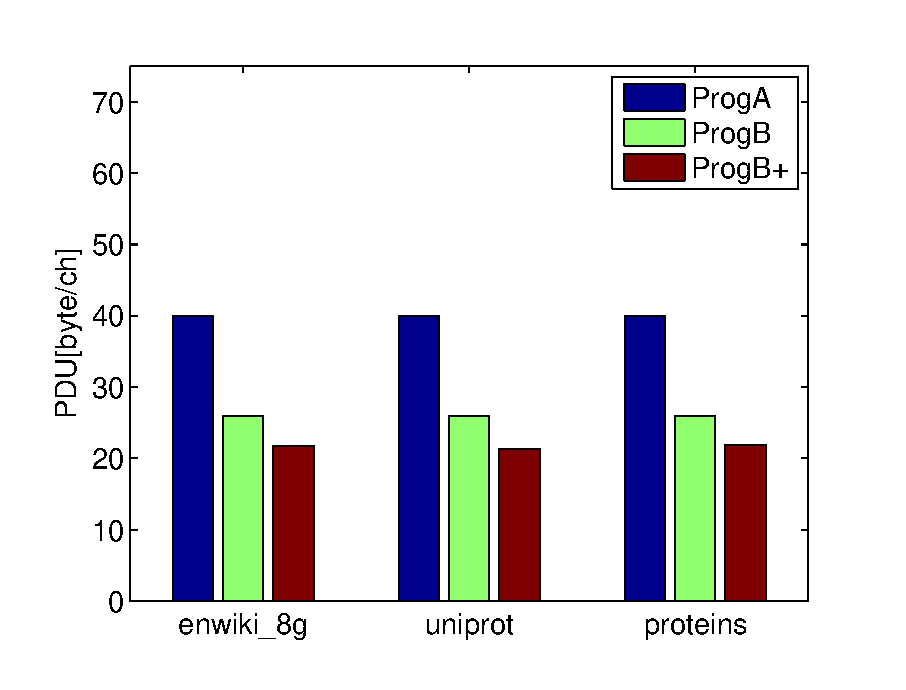
\includegraphics[width = 0.9\columnwidth]{pdu_cmp}
	}
	\hfil
	\subfigure{
		\label{subfig:iov_cmp}
		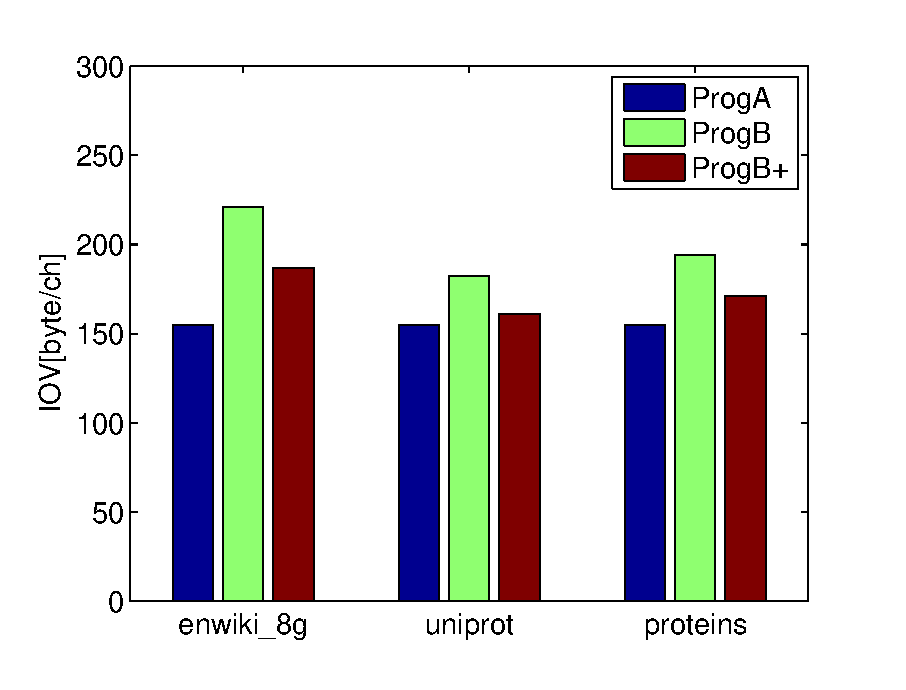
\includegraphics[width = 0.9\columnwidth]{io_cmp}
	}
	\hfil
	\subfigure{
		\label{subfig:ct_cmp}
		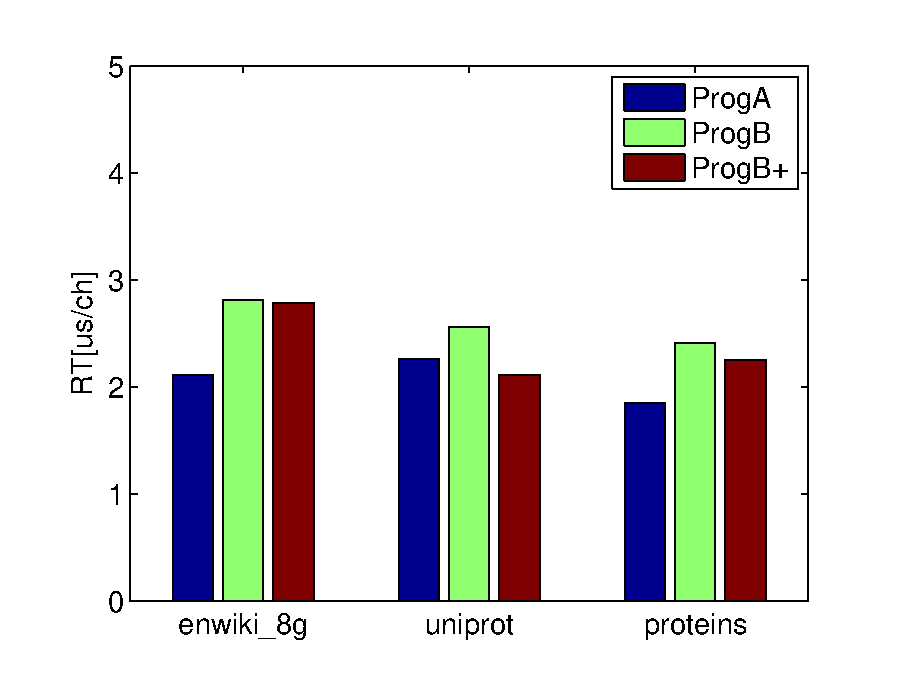
\includegraphics[width = 0.9\columnwidth]{ct_cmp}
	}
	\caption{Performance of ProgA, ProgB and ProgB+ for different corpora.}
	\label{fig:performance_analysis}
\end{figure}

%figure
\begin{figure}[htbp!]
	\centering
	\subfigure{
		\label{subfig:pdu_cmp2}
		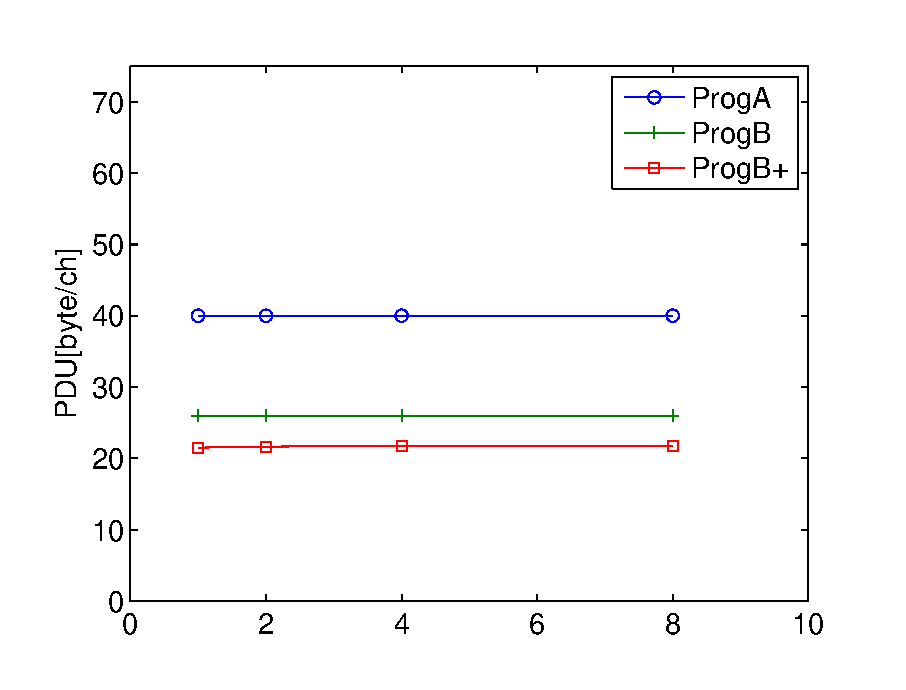
\includegraphics[width = 0.9\columnwidth]{pdu_cmp2}
	}
	\hfil
	\subfigure{
		\label{subfig:iov_cmp2}
		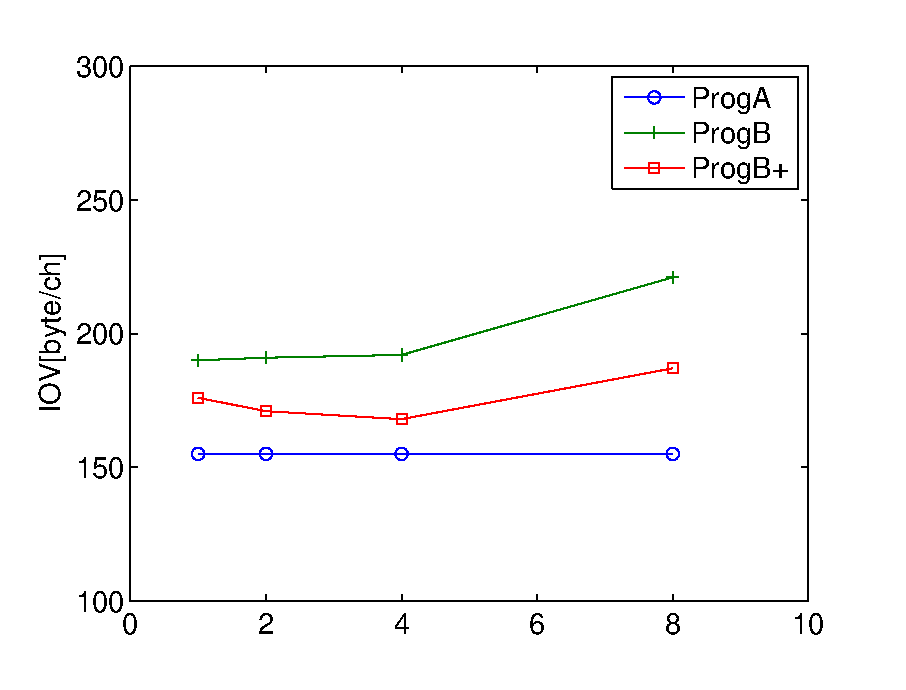
\includegraphics[width = 0.9\columnwidth]{io_cmp2}
	}
	\hfil
	\subfigure{
		\label{subfig:ct_cmp2}
		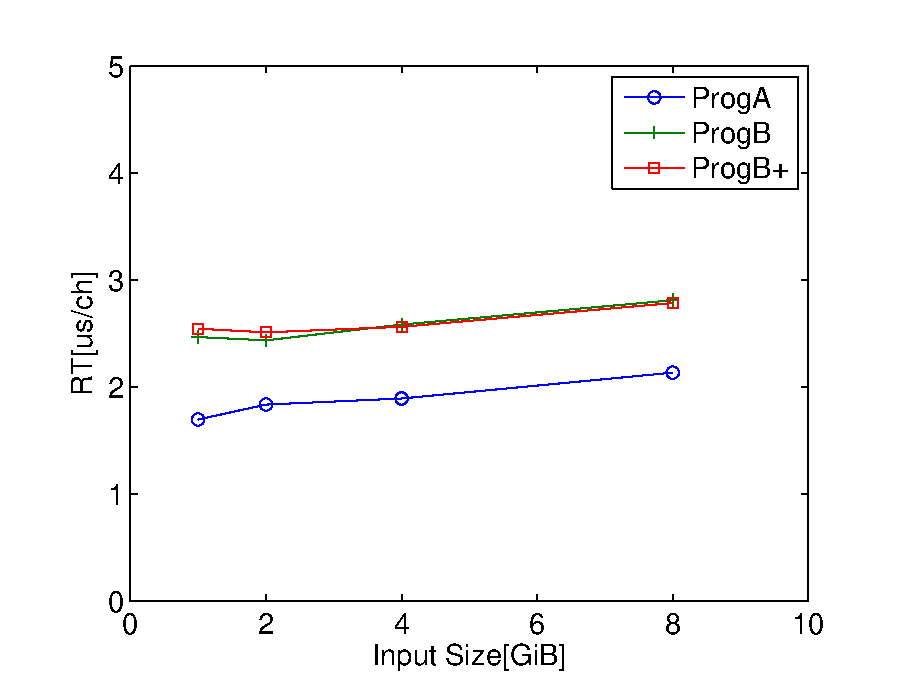
\includegraphics[width = 0.9\columnwidth]{ct_cmp2}
	}
	\caption{Performance of ProgA, ProgB and ProgB+ for prefixes of "enwiki".}
	\label{fig:performance_analysis2}
\end{figure}
	
	
	
%Table
\renewcommand\arraystretch{1.3}
\begin{table*}
	\caption{A performance comparison of checking the suffix and LCP arrays of S*-type suffixes to checking that of all the suffixes.}
	\label{tbl:2}
	\centering
	\begin{tabular}{|l|c|c|c|c|c|c|c|c|c|c|c|c|}
		\hline
		\multirow{2}{*}{dataset} & \multicolumn{3}{|c|}{\# of suffixes} & \multicolumn{3}{|c|}{PDU} & \multicolumn{3}{|c|}{IOV} & \multicolumn{3}{|c|}{RT} \\\cline{2-13}
						 & S*-type & all & ratio & S*-type & all & ratio & S*-type & all & ratio & S*-type & all & ratio \\\hline
		enwiki\_1g & 329810376 & 1073741824 & 0.31 & 15.67 & 40 & 0.39 & 89.94 & 155 & 0.58 & 1.05 & 1.70 & 0.62 \\\hline
		enwiki\_2g & 650901939 & 2147483648 & 0.30 & 15.41 & 40 & 0.39 & 89.18 & 155 & 0.58 & 1.22 & 1.85 & 0.66 \\\hline
		enwiki\_4g & 1301327878 & 4294967296 & 0.30 & 15.45 & 40 & 0.39 & 89.14 & 155 & 0.58 & 1.19 & 1.89 & 0.63 \\\hline
		enwiki\_8g & 2586471839 & 8589934592 & 0.30 & 15.35 & 40 & 0.38 & 88.80 & 155 & 0.57 & 1.33 & 2.14 & 0.62 \\\hline	
		uniprot & 829262945 & 3028811776 & 0.27 & 13.94 & 40 & 0.35 & 83.80 & 155 & 0.54 & 1.04 & 2.26 & 0.46 \\\hline
		proteins & 379092002 & 1184366592 & 0.32 & 16.21 & 40 & 0.41 & 92.29 & 155 & 0.60 & 1.14 & 1.85 & 0.62	\\\hline
		mean & 1012811163 & 3189156522 & 0.30 & 15.34 & 40 & 0.38 & 88.86 & 155 & 0.57 & 1.16 & 1.95 & 0.60 \\\hline
	\end{tabular}
\end{table*}

%It is identified that both programs heavily rely on the performance of the external memory sorter in use. A potential candidate for improving their speed is to adapt a GPU-based multi-way sorter~(e.g.,~\cite{Leischner2010, Davidson2012}) for sorting massive data using external memory. By the aid of these fast sorting algorithms, the throughputs of the programs are expected to nearly approach the I/O bandwidth. Besides, the first two steps of Algorithm~\ref{alg:1} are independent of each other and thus can be executed in parallel for acceleration. This technique can be also applied to check the suffix and LCP arrays of the LMS suffixes in Algorithm~\ref{alg:3}.

%Currently, for Algorithm~\ref{alg:3}, step 2 constitutes the space bottleneck. It is worthy of mentioning that this step produces a copy of the suffix and LCP array during the inducing and checking processes. Actually, given that $\Sigma$ is of a constant size and $sa/lcp$ are known already, we can simply scan the input $sa/lcp$ to perform the inducing process and compare each induced suffix/LCP value with that in the given $sa/lcp$ to perform the checking process, resulting in less space consumption. To the end, we must maintain a read pointer for each suffix/LCP bucket in $sa/lcp$ to scan elements in sequence.

The next experiment is to compare our programs with that of two solutions for building the suffix and LCP arrays as below, where either of them combines an existing suffix sorter with an LCP builder.

\begin{enumerate} [solut{i}on 1]
	\item Use eSAIS for building SA and the sequential version of Sparse-$\phi$~\cite{Karkkainen2016} for building LCP array.
	
	\item Use pSAscan~\cite{Karkkainen2015} for building SA and the parallel version of Sparse-$\phi$ for building LCP array.
\end{enumerate}

 We select eSAIS and pSAscan because they are currently the fastest sequential and parallel SA construction algorithms available to us. Also, Sparse-$\phi$ is the fastest LCP array construction algorithm among those ever reported. A runtime breakdown of the programs for these solutions on the prefixes of "enwiki" is given in Table~\ref{tbl:3}. As can be seen, the program for solution 2 is about two times faster than that for solution 1 and twice as fast as ProgA, which is mainly owing to the high speed of pSAscan. However, it is worthy of pointing out that both pSAscan and Sparse-$\phi$ are of the time and I/O complexity proportional to $n^2/M$. This is much higher than eSAIS and our checking algorithms, and thus poses a limitation to their scalability. As reported in~\cite{Karkkainen2015}, when the input string length is considerably greater than the internal memory size, eSAIS is more quickly and I/O efficient than pSAscan. We can see from Table~\ref{tbl:3} that, the time consumption of constructing the SA for "enwiki\_8g" is doubled as that of constructing the SA for "enwiki\_1g" by means of pSAscan.
 

%Table
\renewcommand\arraystretch{1.3}
\begin{table*}[h]
	\caption{A runtime comparison between the programs for two construction solutions and the proposed algorithms.}
	\label{tbl:3}
	\centering
	\begin{tabular}{|c|c|c|c|c|c|c|c|c|}
		\hline
		\multirow{2}{*}{dataset} & \multicolumn{3}{|c|}{solution 1} & \multicolumn{3}{c|}{solution 2} & \multirow{2}{*}{ProgA} & \multirow{2}{*}{ProgB+} \\\cline{2-7}
		 & eSAIS & sequential sparse-$\phi$ & total & pSAscan & parallel sparse-$\phi$ & total & & \\\hline
		enwiki\_1g & 2.21 & 0.61 & 2.82 & 0.39 & 0.59 & 0.98 & 1.70 & 2.54 \\\hline
		enwiki\_2g & 2.63 & 0.53 & 3.16 & 0.47 & 0.53 & 1.00 & 1.84 & 2.51 \\\hline
		enwiki\_4g & 2.90 & 0.63 & 3.53 & 0.59 & 0.40 & 0.99 & 1.89 & 2.56 \\\hline
		enwiki\_8g & 3.02 & 0.63 & 3.65 & 0.83 & 0.45 & 1.28 & 2.13 & 2.79 \\\hline
	\end{tabular}
\end{table*}



\subsection{Discussion}

There are still several ways to enhance the performance of our programs. Firstly, it was observed that our programs suffer from a bottleneck when sorting massive data in external memory. For implementation simplicity, we currently use the container provided by the STXXL library to perform the sorting task without designing a specific sorter. It is possible to speed up the sorting process by means of the high-performance radix-sort algorithms proposed on GPU-based computation platforms. Secondly, Method B checks the suffix and LCP arrays using the induced sorting principle. At the time of writing this paper, the existing IS-based suffix/LCP array construction algorithms are not capable of fully using the available computation resources. We are now devoted to designing IS-based construction algorithms scalable for running in parallel environments. This work may also improve the implementation design of Algorithm~\ref{alg:2}. 

Method A has a higher versatility compared to the existing construction algorithms, it can be employed to check any set containing one or multiple pairs of lexicographically neighboring or non-neighboring suffixes. This feature can be applied to various scenarios. For example, sometimes the consistency of a suffix/LCP array may be broken due to hardware malfunctions or human errors. If the backup of the corrupted data is not available and it is too time-consuming to rebuild the whole array, then we can locate the bad areas quickly using Algorithm~\ref{alg:1} and restore the partial SA for each area by calling a sparse SA construction algorithm. Another example is to check the correctness of a sparse SA. Because the number of suffixes in a sparse SA is commonly much smaller than the number of suffixes in the corresponding SA, it is expected that a substantial improvement in time, space and I/O volume can be achieved when performing verification using Algorithm~\ref{alg:1}.


\section{Conclusions} \label{sec:conclusion}

In this paper, we propose two methods for probabilistically checking the given suffix and LCP arrays. Theoretically, the external-memory algorithms designed by these methods have better time and I/O complexities compared to the existing fastest construction algorithms. Our experimental results indicate that the programs for Algorithm~\ref{alg:2} designed by Method B run slower than that for Algorithm~\ref{alg:1} designed by Method A, but they are much more space-efficient than the latter. As discussed in Section~\ref{sec:experiment}, there is still a great potential for enhancing the performance of our programs. For future work, we are now attempting to redesign the sorting and inducing process in our implementations to make them competitive with the state-of-the-art parallel construction algorithms. 

From our perspective, a checker should be not only fast but also versatile. As a common practice, we usually check an array derived from a builder by literally comparing it with the one produced by another builder. However, this is not feasible in all the cases, because, for example, an algorithm for constructing infinite-order array can not be directly used to check a finite-order array and vise versa. On the contrary, our first method can be generalized to check the correctness of the lexical order and the LCP values of one or multiple pairs of suffixes starting at any positions of input string. This makes it possible to trivially adapt Algorithm~\ref{alg:1} for verifying a sparse or finite-order SA together with the corresponding LCP array.

\appendices
\section{Overview on the Induction Phase} \label{sec:appendix}

Recall that the lexical order of two suffixes starting with $x[i]$ and $x[j]$ can be determined by sequentially comparing their characters until finding a position $k$ such that $x[i, i + k) = x[j, j + k)$ and $x[i + k] \ne x[j + k]$. In other words, we have ${\sf suf}(i) < {\sf suf}(j)$ if (1) $x[i] < x[j]$~$(k = 0)$ or (2) $x[i] = x[j]$ and ${\sf suf}(i + 1) < {\sf suf}(j + 1)$~$(k > 0)$; otherwise, ${\sf suf}(i) > {\sf suf}(j)$. This rule is used by the IS-based SA construction algorithms to sort suffixes during the induction phase:

\begin{enumerate}[S1]
	\item 
	Clear S-type sub-buckets in $sa$. Scan $sa^*$ leftward and insert each element into current rightmost empty position in the corresponding S-type sub-bucket.
	
	\item 
	Clear L-type sub-buckets in $sa$ and insert $n - 1$ into the leftmost position in ${\sf sa\_bkt_L}(x[n - 1])$. Scan $sa$ rightward with $i$ increasing from $0$ to $n - 1$. For each scanned non-empty $sa[i]$ with $t[sa[i] - 1] = 0$, insert $sa[i] - 1$ into current leftmost empty position in ${\sf sa\_bkt_L}(x[sa[i] - 1])$.
	
	\item
	Clear S-type sub-buckets in $sa$. Scan $sa$ leftward with $i$ decreasing from $n - 1$ to $0$. For each scanned non-empty $sa[i]$ with $t[sa[i] - 1] = 1$, insert $sa[i] - 1$ into current rightmost empty position in ${\sf sa\_bkt_S}(x[sa[i] - 1])$.
	
\end{enumerate}

In brief, assume $sa^*$ is already known, S1 inserts all the S*-type suffixes into $sa$ in their lexical order. Then, S2-S3 induce the order of L-type and S-type suffixes from those already sorted in $sa$, respectively, where the relative order of two suffixes induced into the same sub-bucket matches their insertion order according to the rule stated above. To be more specific, we show in Fig.~\ref{fig:example2} a running example of the induction phase. 

As depicted, the input string $x$ contains 6 S*-type suffixes sorted in line 3. When finished inserting the S*-type suffixes in lines 5-6, we first find the head of each L-type sub-bucket (marked by the symbol $\wedge$) and insert ${\sf suf}(13)$ into $sa$. Notice that ${\sf suf}(13)$ consists of only one character, it must be the smallest L-type suffixes starting with $1$. Thus, we put ${\sf suf}(13)$ into the leftmost position in ${\sf sa\_bkt_L}(1)$ in line 8. Then, we scan $sa$ from left to right for inducing the order of all the L-type suffixes. In lines 10-11, when visiting $sa[0] = 13$ (marked by the symbol $@$), we check the type array $t$ to find $x[12] = 2$ is L-type and hence insert ${\sf suf}(12)$ into current leftmost empty position in ${\sf sa\_bkt_L}(2)$. Similarly, in lines 12-13, we visit the next scanned item $sa[1] = 11$ and see that $t[10] = 0$, thus we place ${\sf suf}(10)$ into the current head of ${\sf sa\_bkt_L}(3)$. Following this way, we get all the L-type suffixes sorted in $sa$. After that, we first find the end of each S-type sub-bucket in lines 25-26 and scan $sa$ leftward for inducing the order of all the S-type suffixes in lines 27-40. When visiting $sa[13] = 2$, we see $x[1]$ is S-type and thus put ${\sf suf}(1)$ into current rightmost empty position in ${\sf sa\_bkt_S}(1)$. Then, at $sa[12] = 8$, we see $x[7] = 1$ is S-type and thus put ${\sf suf}(7)$ into current rightmost empty position in ${\sf sa\_bkt_S}(1)$. To repeat scanning $sa$ in this way, we get all the S-type suffixes sorted in $sa$. 

The work presented in~\cite{Fischer11} describes how to compute the LCP array during the execution of S2-S3. Given two suffixes placed at the neighboring positions in $sa$, their LCP-value can be computed according to one of the following two cases with regard to whether or not they are inserted into the same sub-bucket: if yes, then the LCP-value of them is one greater than that of the two suffixes from which inducing them; otherwise, the LCP-value of them is equal to zero. In this way, we can determine $lcp[i]$ immediately after the computation of $sa[i]$. The problem here is how to obtain the LCP-value of these inducing suffixes, which is modeled as a range minimum query in~\cite{Fischer11} and can be easily answered within $\mathcal{O}(1)$ time using $\mathcal{O}(\|\Sigma\|)$ space. For example, when scanning from $sa[0]$ to $sa[5]$ in lines 10-21 of Fig.~\ref{fig:example2}, we induce ${\sf suf}(12)$ and ${\sf suf}(6)$ into the neighboring positions in ${\sf sa\_bkt_L(2)}$. During the scan of $sa[0, 5]$, if we keep recording the minimal of $lcp(0, 5]$ in a variable, then we can obtain the LCP-value of the inducing suffixes ${\sf suf}(13)$ and ${\sf suf}(5)$ from this variable when putting ${\sf suf}(6)$ into $sa$. 

\begin{figure}
	\centering
	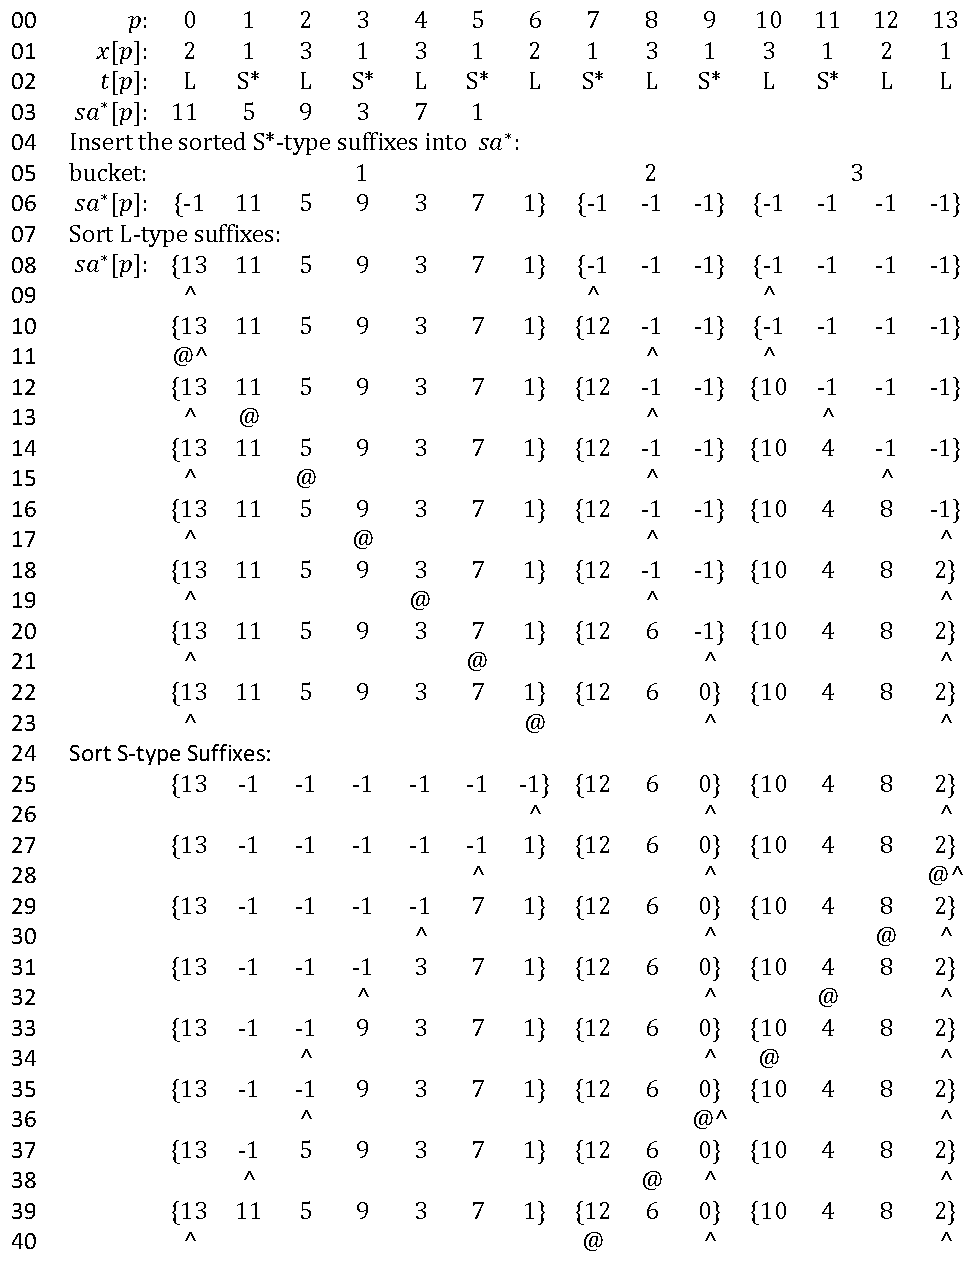
\includegraphics[width = 0.9\columnwidth]{example2}

	\caption{An Example for computing the suffix and LCP arrays during the induction phase. \label{fig:example2}}	
\end{figure}
 
% Bibliography
\bibliographystyle{IEEEtran}
\bibliography{IEEEabrv,bibfile}
	
\end{document}


We are intended for ....

put emphasis on

with the same ease as when

The biggest difference between two is that ...

Toward the end, ...

they are designed to be both easy to interpret on ... and easily traslated into ... (they are designed to be easily implemented in classic external memory models)

Having a ... eliminates .... (random accesses), access ordering

Not only are ..., but 

The fingerprints are calculated on the fly during the scan of x ...

become so good that they are competitive with ...., and in some cases, even outperform them ...

concurrent programming is needed to make sure ....

designed to adapt to an evolving environment

most importantly

exchanges data between the computer presenting the applet and the computer serving it.

carries out sophisticated calculations

Presumably because

make ... capable of ...

greatly improve ... , it was still rather limited, though.


additional performance improvements

close the chapter with ...

gain

which pose ...

integrate with

In this chapter, we will ... how to ... and how to ...


we prefer the comfort of an integrated development environment, ( prefer the low cost of fingerprinting techinques)

space-hungry


begin exploring ... by ...

commnuicate the monmentous advances

extremely simple

check each number is present in the suffix array.

go into much more greater details

stand-alone algorithms for computing suffix arrays only and has been reused to 

invoke/call


the mechanics of ...

If you have done sth, then when you do sth, you end up with ...

depend on the machine on which you will be running the java code ...


alleviate



The second method is invented to overcome the drawback of 

in place of

as to/about

as far as

assign to a variable

stated goals

intermediate steps

tied to the behavior of 

an assortment of 

following the footsteps of 

characters in the input string are processed from left to right

in greater detail

in the  order received


build up a whole new thing from scratch

In the interest of completeness, we briefly discuss the date and time formatting options of the printf method

immediately follow

preceding statement

tuned version


hang on to the object

track down 


invisible to the remainder of the program

put it another way
































